\subsection{Low-Pass Filter Realizability\label{sec:ch6:lpf}}

\subsubsection{Synthesis Task}

\begin{figure}
\centering
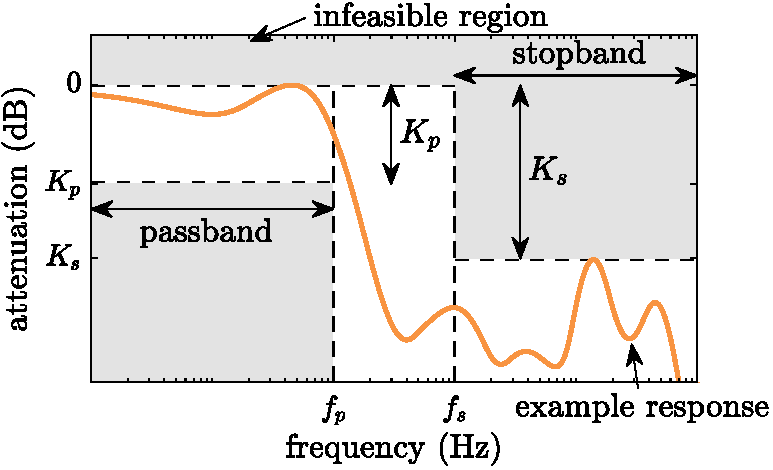
\includegraphics[width=0.6\textwidth]{../ch6/figures/reduced/r_filter_specs}
\caption{Low-pass filter specifications.\label{fig:ch6:filter:specs}}
\end{figure}

The second example is the synthesis of a \glsfirst{LPF}. A LPF attenuates signals above a certain frequency and passes all other signals.
The design specification of a LPF is shown in Fig.~\ref{fig:ch6:filter:specs}.
There are many classical synthesis methods for LPFs such as Butterworth, Chebyshev I, Chebyshev II, Elliptic,  Legendre-Papoulis, etc. \cite{Wanhammar2009a}.
LPFs are also frequently used as examples for evolutionary-based synthesis methods \cite{Das2007a, Gan2010a, Goh2001a, Grimbleby2000a, Koza1997a, Koza2000a, Lohn1999a}.
Here we will try to synthesize four LPFs with their specifications and variable bounds shown in Table~\ref{tb:ch6:lpfspecs}.

\subsubsection{Circuit Structure Space}

The desired circuit structure space is ``all topologies that have up to 7 passive components with an optional connection to the ground''.
Such a space is captured by:
\begin{subequations}
\label{eq:ch6:lib3}
\begin{align}
C &= \{ \xcolor{I}, \xcolor{O}, \xcolor{G}, \xcolor{Z}, \xcolor{N3}, \xcolor{N4}, \xcolor{N5}, \xcolor{N6}, \xcolor{N7}, \xcolor{N8}, \xcolor{N9} \} \\
P &=        \left[ 1\ 1\ 1\ 2\ 3\ 4\ 5\ 6\ 7\ 8\ 9 \right] \\
R_{\min} &= \left[ 1\ 1\ 0\ 1\ 0\ 0\ 0\ 0\ 0\ 0\ 0 \right] \\
R_{\max} &= \left[ 1\ 1\ 1\ 7\ 5\ 4\ 3\ 2\ 2\ 2\ 1 \right]
\end{align}
\end{subequations}

\noindent and includes all the NSCs from Sec.~\ref{sec:ch6:primitive}.
This is very similar to Eqn.~(\ref{eq:ch6:lib2}), except $\xcolor{Z}$ now has up to seven replicates, $\xcolor{G}$ is optional, and some of the $\xcolor{N}x$ maximum replicate numbers have changed based on what is needed for Eqn.~(\ref{eq:ch6:subcatalog:feas}).
The subcircuits for generating practical circuits will be series connections between $\{\xcolor{L},\xcolor{C}\}$ components to replicate the elements typically used in LPFs.
The primitive circuit library then has 5,300 unique graphs and these graphs are expanded to 1,804,496 unique practical circuit graphs (see Table~\ref{tb:ch6:lpf:computational}).

\begin{table}[ht]
\centering
\caption{Computational cost of \nameref{sec:ch6:lpf} example.\label{tb:ch6:lpf:computational}}
\begin{tabular}{rrrr}
\hline \hline
 & Step                   & $t$ (s) & $N$ \\
\hline
\multirow{3}{*}{Circuit generation} & Primitive circuits  & 2,694 & 5,300  \\
 & Practical circuits & 6,330  & 1,804,496  \\
 & Transfer functions & 20,460 & 123,156   \\
 \multirow{4}{*}{Evaluation}        & Task \#1 & 235,810 & 123,156     \\
 & Task \#2 & 80,788 &  38,172   \\
 & Task \#3 & 83,231 & 38,172    \\
 & Task \#4 & 606 & 281    \\
\hline \hline
\end{tabular}
\end{table}

This synthesis task will utilize the template circuit in Fig.~\ref{fig:ch6:template:filter} with parameters $\{\gls{vs},\gls{Rs},R_l\}$ valued at $\{2 \text{V}, 1 \text{k}\Omega, 1 \text{k}\Omega\}$.
Of the 1,804,496 practical circuit graphs, 123,156 were found to have less than 7 components and remain unique transfer functions.
The practical circuit graph representation can be used directly to count the number of components before the transfer function is constructed.

\subsubsection{Results}

\begin{table}[ht]
\centering
%--------------------------------
\begin{subfigure}[t]{\textwidth}
\centering
\begin{tabular}{cccccccc}
\hline \hline
\# & c.f. & \gls{fp} (Hz) & \gls{fs} (Hz) & \gls{Kp} (dB) & \gls{Ks} (dB) & \gls{inductance} bounds (H) & $C$ bounds (F) \\
\hline
1 & \cite{Lohn1999a, Goh2001a} & 925 & 3200 & 3.01 & 22.0 & $\left[0.1\text{m}, 1.5\right]$ & $\left[0.1\text{p}, 200\mu\right]$ \\ % (6)
2 & \cite{Gan2010a} & 1000 & 2000 & 1.00 & 60.0 & $\left[0.01\text{m}, 10\right]$ &$ \left[0.1\text{p}, 100\mu\right]$ \\ % (11) 
3 & \cite{Das2007a} & 800 & 2000 & 0.60 & 68.0 & $\left[0.1\text{m}, 1\right]$ & $\left[100\text{p}, 1\mu\right]$ \\ % ()
4 & \cite{Lohn1999a, Goh2001a} & 1000 & 2000 & 0.01 & 63.5 & $\left[0.1\text{m}, 1.5\right]$ & $\left[0.1\text{p}, 200\mu\right]$ \\
\hline \hline
\end{tabular}
\caption{Specifications.}
\end{subfigure}
%--------------------------------
\begin{subfigure}[t]{\textwidth}
\centering
\begin{tabular}{cccc}
\hline \hline
\# & \# feasible & \% feasible & $\min n_c$ \\
\hline
1 & 38172 & 30.99 & 3   \\ % (6)
2 & 280 & 0.23 & 6 \\ % (11) 
3 & 197 & 0.16 & 6 \\ % ()
4 & 0 & 0 & $>7$ \\
\hline \hline
\end{tabular}
\caption{Results.}
\end{subfigure}

\caption[\nameref{sec:ch6:lpf} specifications and results.]{Summary of \nameref{sec:ch6:lpf} specifications and results.\label{tb:ch6:lpfspecs}}

%--------------------------------
\end{table}

The results for this example are summarized in Table~\ref{tb:ch6:lpfspecs} with the number of synthesized feasible circuits, the percentage of circuit topologies that were feasible after sizing, and the minimum number of components needed to satisfy the synthesis specifications.
The tasks had increasingly more difficult to satisfy specifications.

% study 1
\begin{figure}
\centering

\begin{subfigure}[t]{0.16\textwidth}
\centering
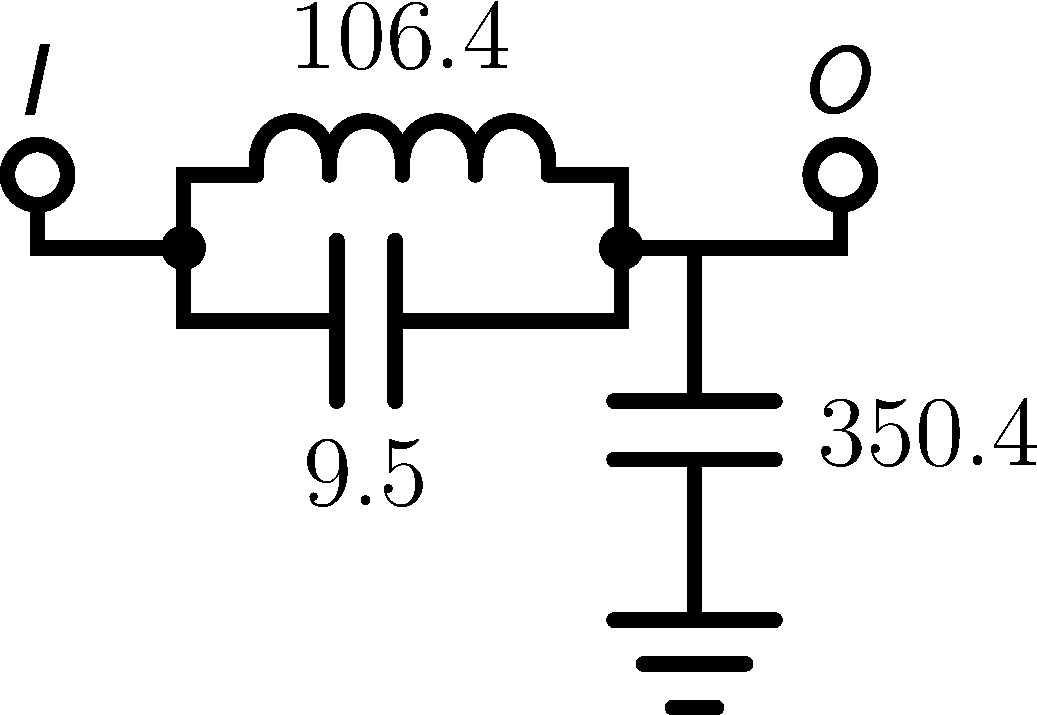
\includegraphics[scale = 0.14]{../ch6/figures/lpf1_circuit1}
\caption{\label{fig:lpf1_circuita}}
\end{subfigure}%
\begin{subfigure}[t]{0.16\textwidth}
\centering
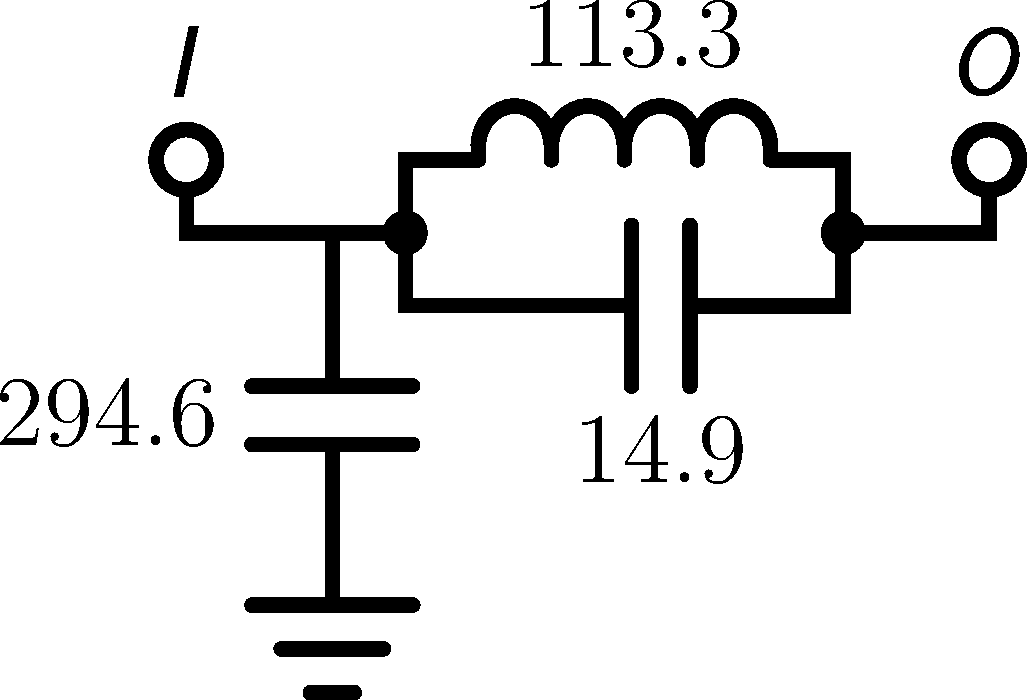
\includegraphics[scale = 0.14]{../ch6/figures/lpf1_circuit2}
\caption{\label{fig:lpf1_circuitb}}
\end{subfigure}%
\begin{subfigure}[t]{0.16\textwidth}
\centering
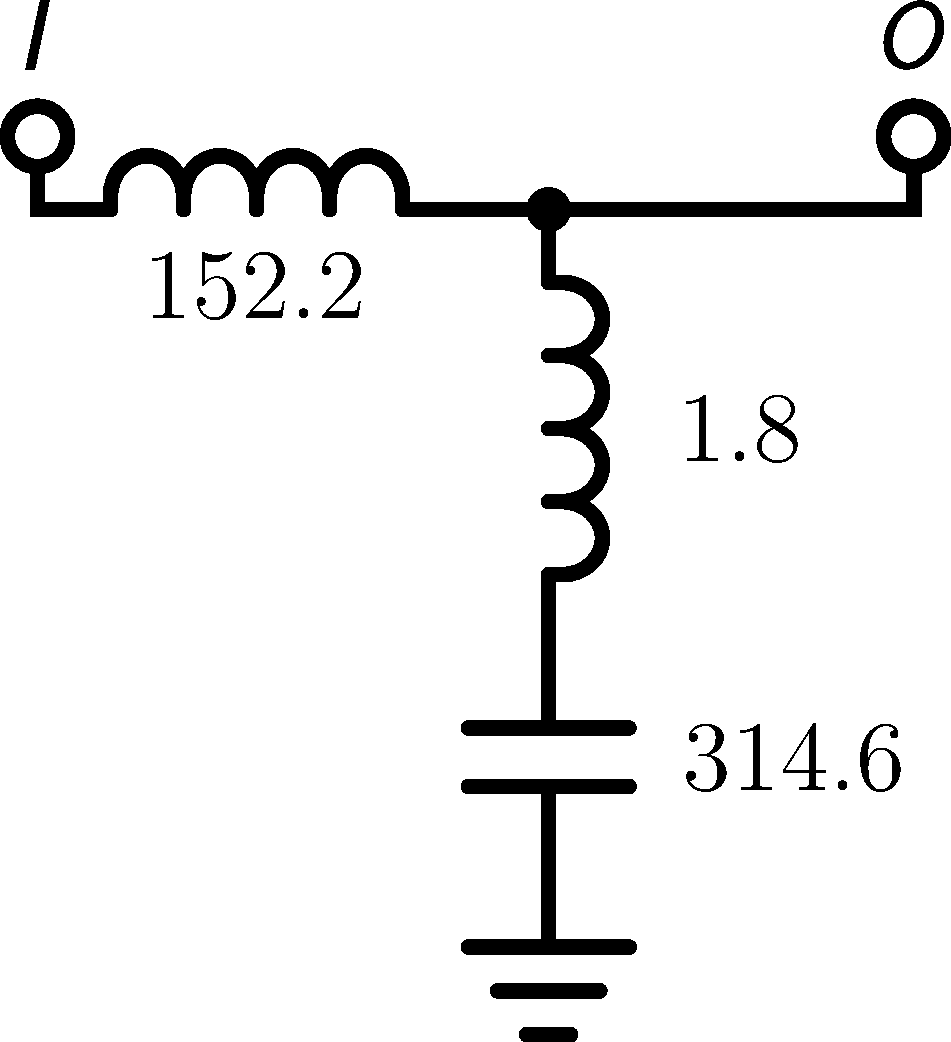
\includegraphics[scale = 0.14]{../ch6/figures/lpf1_circuit4}
\caption{\label{fig:lpf1_circuitc}}
\end{subfigure}%
\begin{subfigure}[t]{0.16\textwidth}
\centering
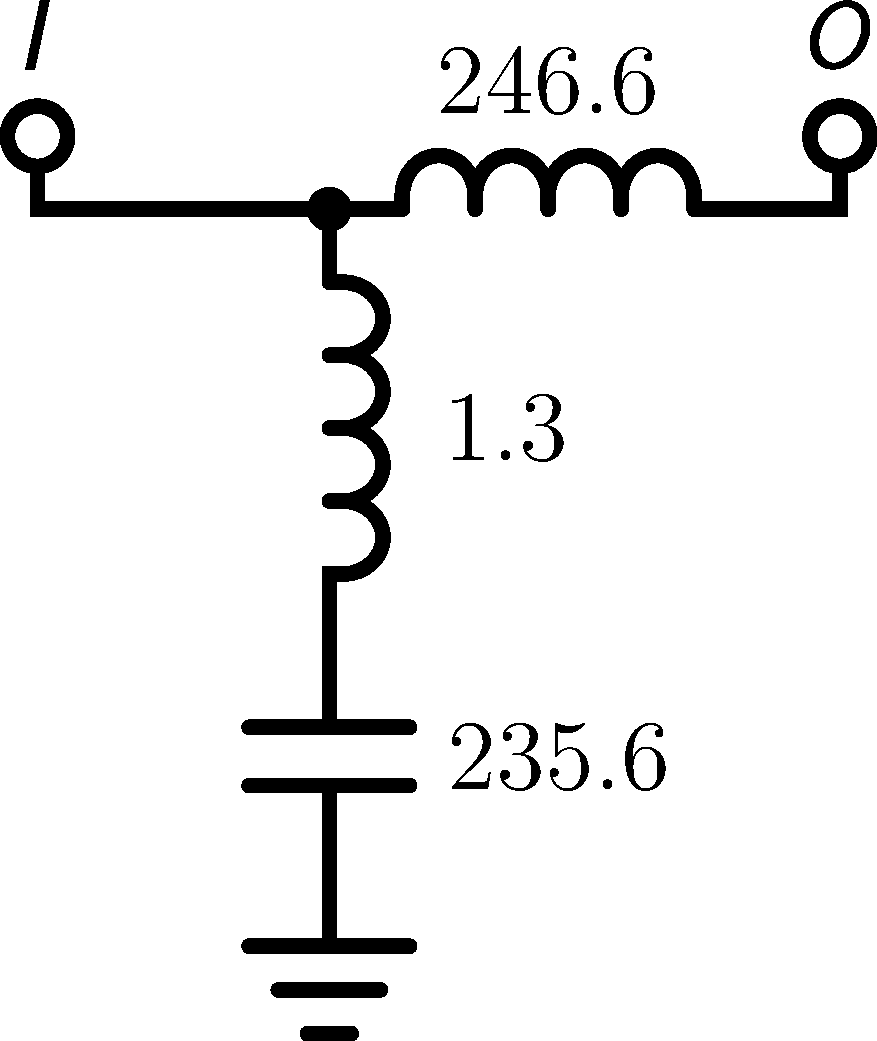
\includegraphics[scale = 0.14]{../ch6/figures/lpf1_circuit5}
\caption{\label{fig:lpf1_circuitd}}
\end{subfigure}%
\begin{subfigure}[t]{0.16\textwidth}
\centering
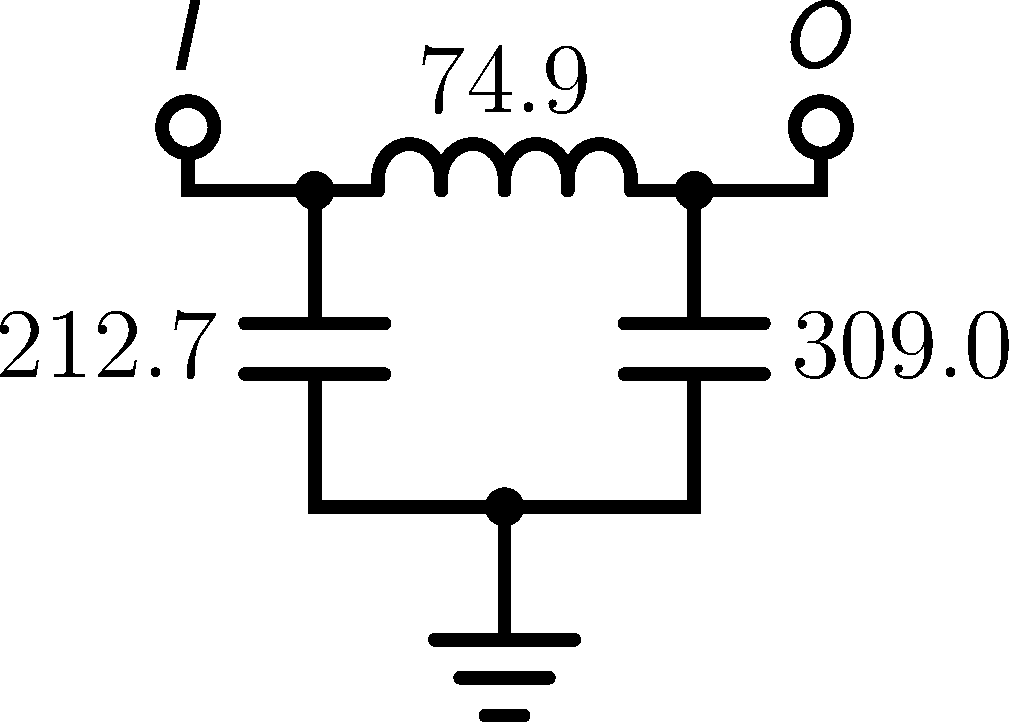
\includegraphics[scale = 0.14]{../ch6/figures/lpf1_circuit3}
\caption{\label{fig:lpf1_circuite}}
\end{subfigure}%
\begin{subfigure}[t]{0.16\textwidth}
\centering
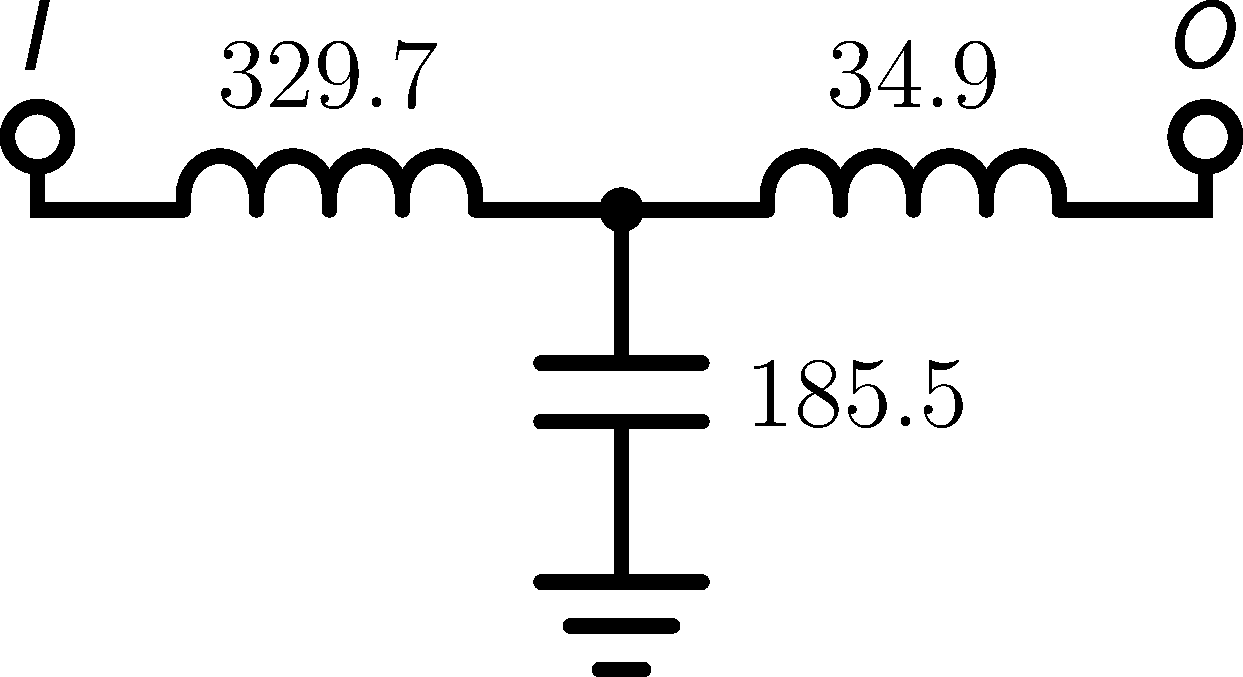
\includegraphics[scale = 0.14]{../ch6/figures/lpf1_circuit6}
\caption{\label{fig:lpf1_circuitf}}
\end{subfigure}%
\vspace{0.06in}
\begin{subfigure}[t]{\textwidth}
\centering
% 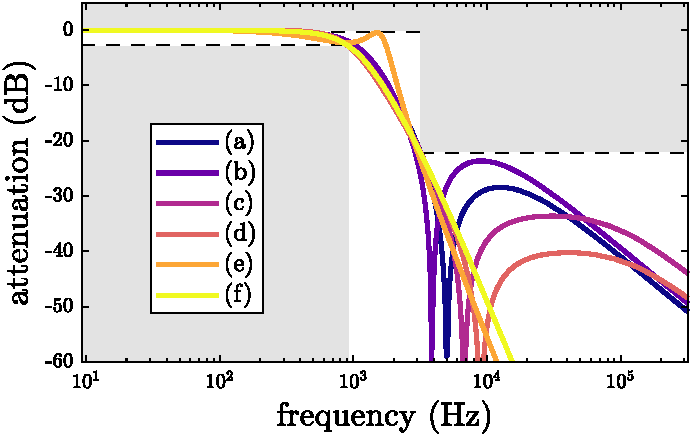
\includegraphics[width=\textwidth]{../ch6/figures/lpf1_magnitude}
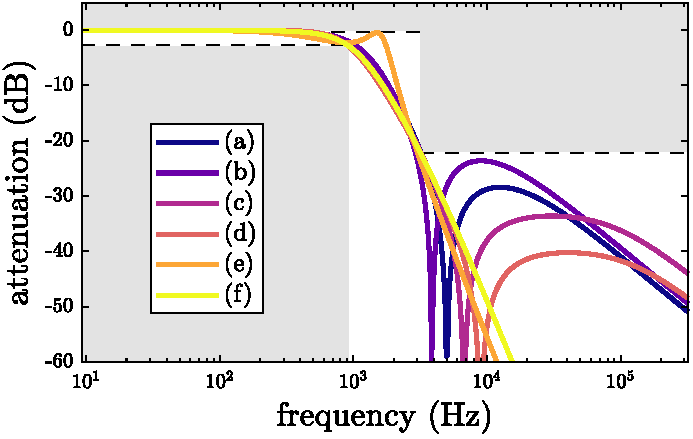
\includegraphics[width=0.5\textwidth]{../ch6/figures/reduced/r_lpf1_magnitude}
\caption{\label{fig:lpf1_magnitude}}
\end{subfigure}%

\caption[All feasible, minimum complexity circuits and attenuation responses for \nameref{sec:ch6:lpf} task \#1.]{All feasible, minimum complexity circuits and attenuation responses for \nameref{sec:ch6:lpf} task \#1 (units are mH and nF).\label{fig:lpf1}}

\end{figure}

The first study is based on examples in Refs.~\cite{Lohn1999a, Goh2001a}, and the specifications were chosen such that they could be satisfied using a third-order Butterworth filter \cite{Lohn1999a}.
This implies that there should be at least one three-component topology that satisfies the specifications (ignoring the variable bounds).
In fact, there are six different three-component topologies that satisfy the requirements, all shown in Figs.~\ref{fig:lpf1_circuita}--\ref{fig:lpf1_circuitf}.
The circuits in Fig.~\ref{fig:lpf1_circuita} and Fig.~\ref{fig:lpf1_circuitb} are topologically similar to one another, as well as Fig.~\ref{fig:lpf1_circuitc} and Fig.~\ref{fig:lpf1_circuitd}.
The other two are well known topologies; Fig.~\ref{fig:lpf1_circuite} is a $\pi$-section, and Fig.~\ref{fig:lpf1_circuitf} is a T-section.
Their attenuation responses are shown in Fig.~\ref{fig:lpf1_magnitude}; all responses are within the specifications.

% new paragraph
The best circuit for task \#1 found in Ref.~\cite{Goh2001a} is Fig.~\ref{fig:lpf1_circuitb}; thus, their evolutionary approach did find one of the minimum-complexity circuits. 
The best circuit from Ref.~\cite{Lohn1999a} had seven components; it is not reported as it is not a minimum-complexity topology.
Since enumeration was used, we can look at the likelihood that certain topologies would have been feasible.
For topologies with up to seven components, 30.99\% of the topologies are feasible (see Table~\ref{tb:ch6:nc:feasible:task1} for the percentage for each complexity level).

\begin{table}
\centering
\caption{Task \#1 feasible vs. total number of circuits for different complexity levels.\label{tb:ch6:nc:feasible:task1}}
\begin{tabular}{rrrr}
\hline \hline
& \multicolumn{2}{c}{Circuits} & \\
$n_c$ & Feasible & Total & \%  \\
\hline
1 & 0 & 2 & 0.0 \\
2 & 0 & 12 & 0.0 \\
3 & 6 & 60 & 10.0 \\
4 & 62 & 338 & 18.3 \\
5 & 534 & 2,192 & 24.4 \\
6 & 4,240 & 14,685 & 28.9 \\
7 & 33,330 & 105,867 & 31.5 \\
\hline \hline
\end{tabular}
\end{table}

% study 2
\begin{figure}
\centering
\begin{subfigure}[t]{0.25\textwidth}
\centering
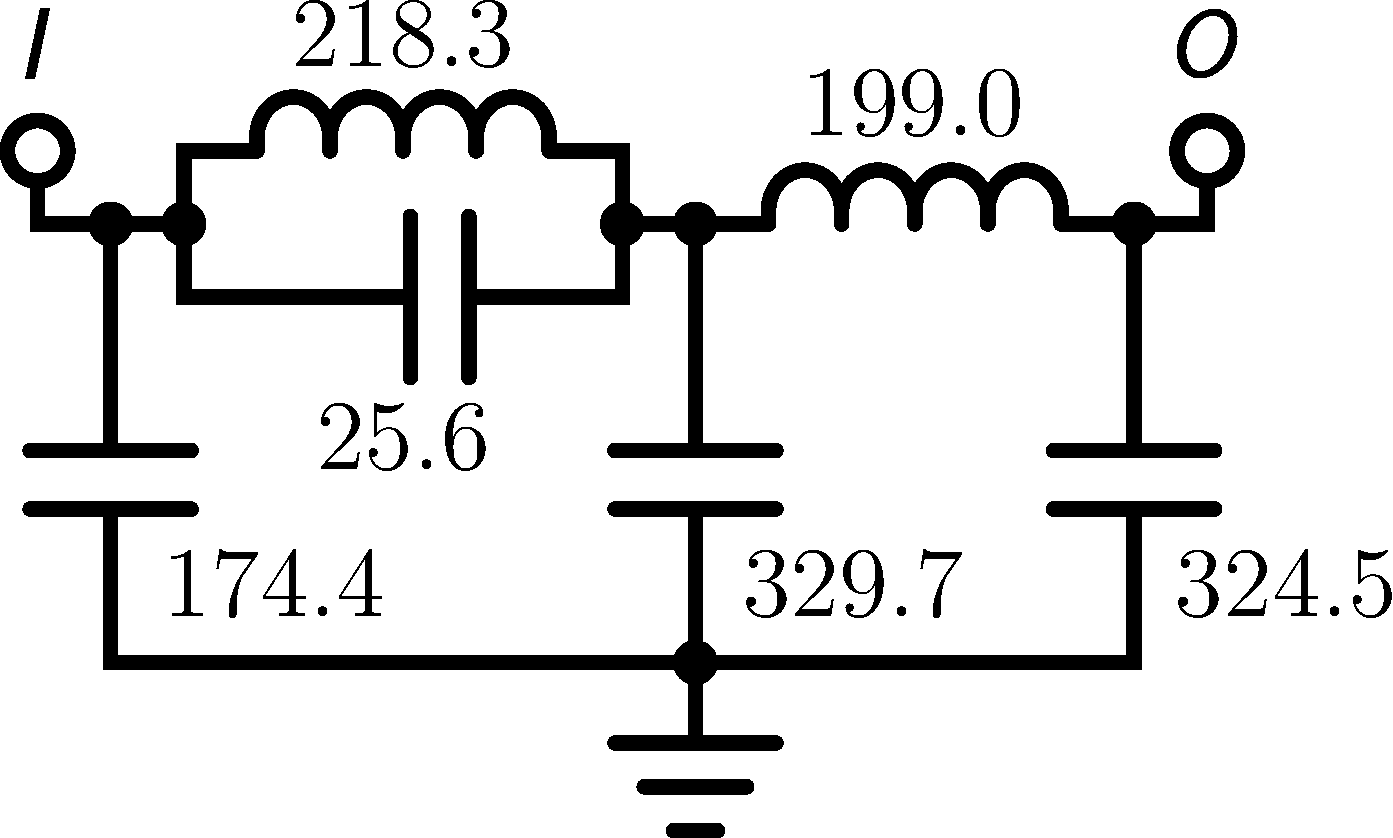
\includegraphics[scale = 0.14]{../ch6/figures/lpf2_circuit1}
\caption{\label{fig:lpf2_circuita}}
\end{subfigure}%
\begin{subfigure}[t]{0.25\textwidth}
\centering
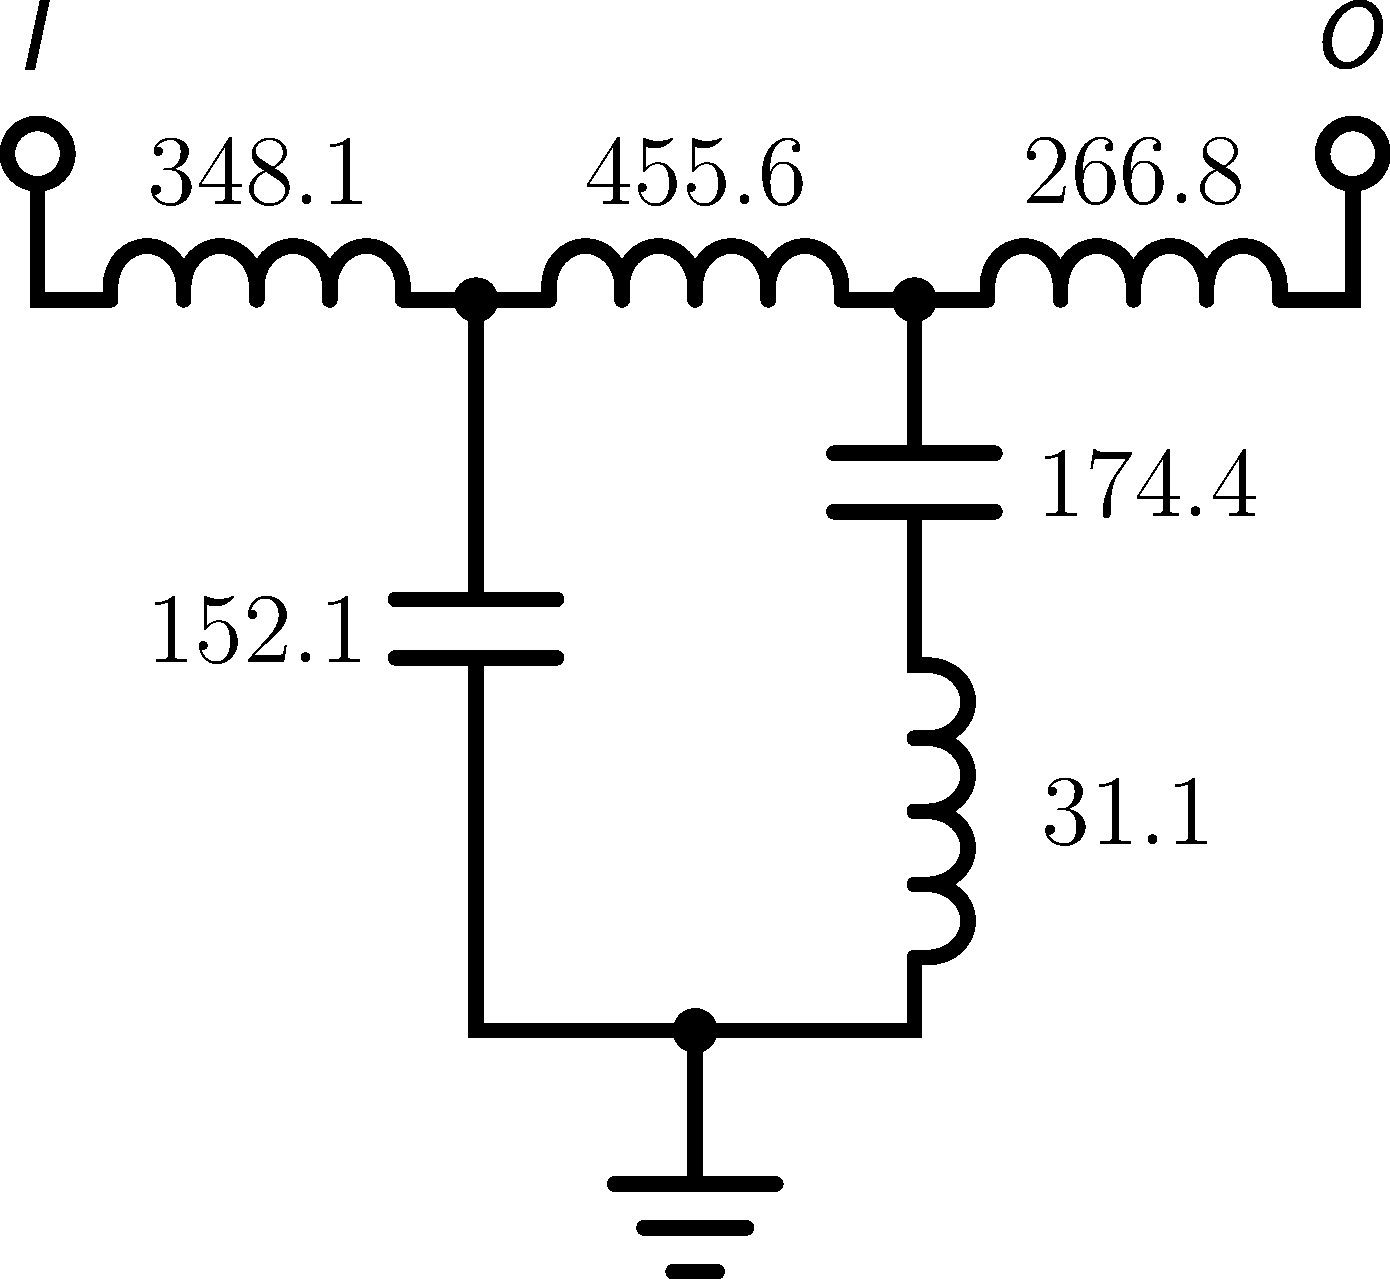
\includegraphics[scale = 0.14]{../ch6/figures/lpf2_circuit2}
\caption{\label{fig:lpf2_circuitb}}
\end{subfigure}%
% \vspace{0.06in}
\begin{subfigure}[t]{0.5\textwidth}
\centering
% 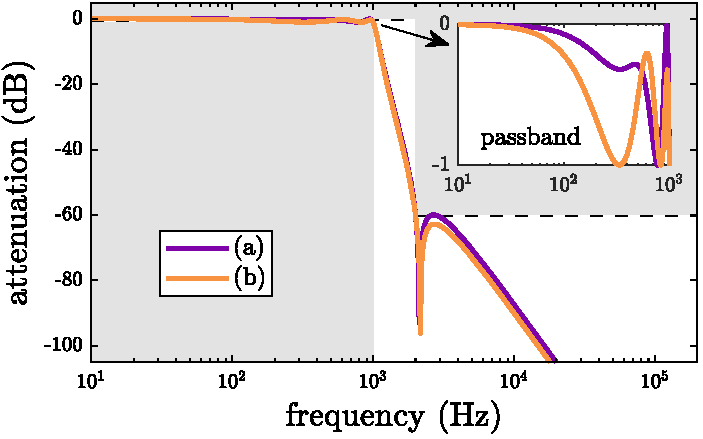
\includegraphics[width=\textwidth]{../ch6/figures/lpf2_magnitude}
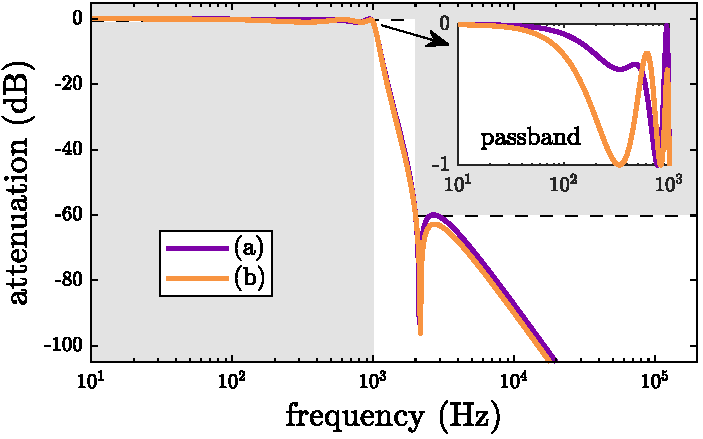
\includegraphics[width=\textwidth]{../ch6/figures/reduced/r_lpf2_magnitude}
\caption{\label{fig:lpf2_magnitude}}
\end{subfigure}%

\caption[Select feasible, minimum complexity circuits and attenuation responses for \nameref{sec:ch6:lpf} task \#2.]{Select feasible, minimum complexity circuits and attenuation responses for \nameref{sec:ch6:lpf} task \#2 (units are mH and nF).\label{fig:lpf2}}

\end{figure}

The specifications for task \#2 are more stringent.
Because of this, we can take the 38,204 feasible circuits from task \#1 as the starting set of circuits since any circuit that is not feasible in task \#1 will not be feasible in task \#2.
From this, only 280 circuits are found to be feasible with the minimum $n_c$ being six components.
Two of the eleven minimum-complexity circuits are shown in Figs.~\ref{fig:lpf2_circuita}--\ref{fig:lpf3_circuitb}.
Their attenuation responses are shown in Fig.~\ref{fig:lpf2_magnitude} (note the magnified region to highlight constraint satisfaction in the passband).

In Ref.~\cite{Gan2010a}, the reported circuit had eight components.
A direct comparison is not a fair assessment, as their study limited the preferred (discrete) component values (E12 series).
However, we can see that Fig.~\ref{fig:lpf2_circuita} is the same as their reported topology when \textsf{C4} and \textsf{C5} are removed.
An alternative complexity metric is the number of inductors as inductors can be bulky, heavy, and expensive compared to capacitors \cite{Wanhammar2009a}.
Under this metric, Fig.~\ref{fig:lpf2_circuita} is the minimum inductor solution (with two alternatives).
A similar discussion can be had with the task \#1 results, where only one inductor is needed in three of the circuits, such as in Fig.~\ref{fig:lpf1_circuita}.

% study 3
\begin{figure}
\centering
\begin{subfigure}[t]{0.25\textwidth}
\centering
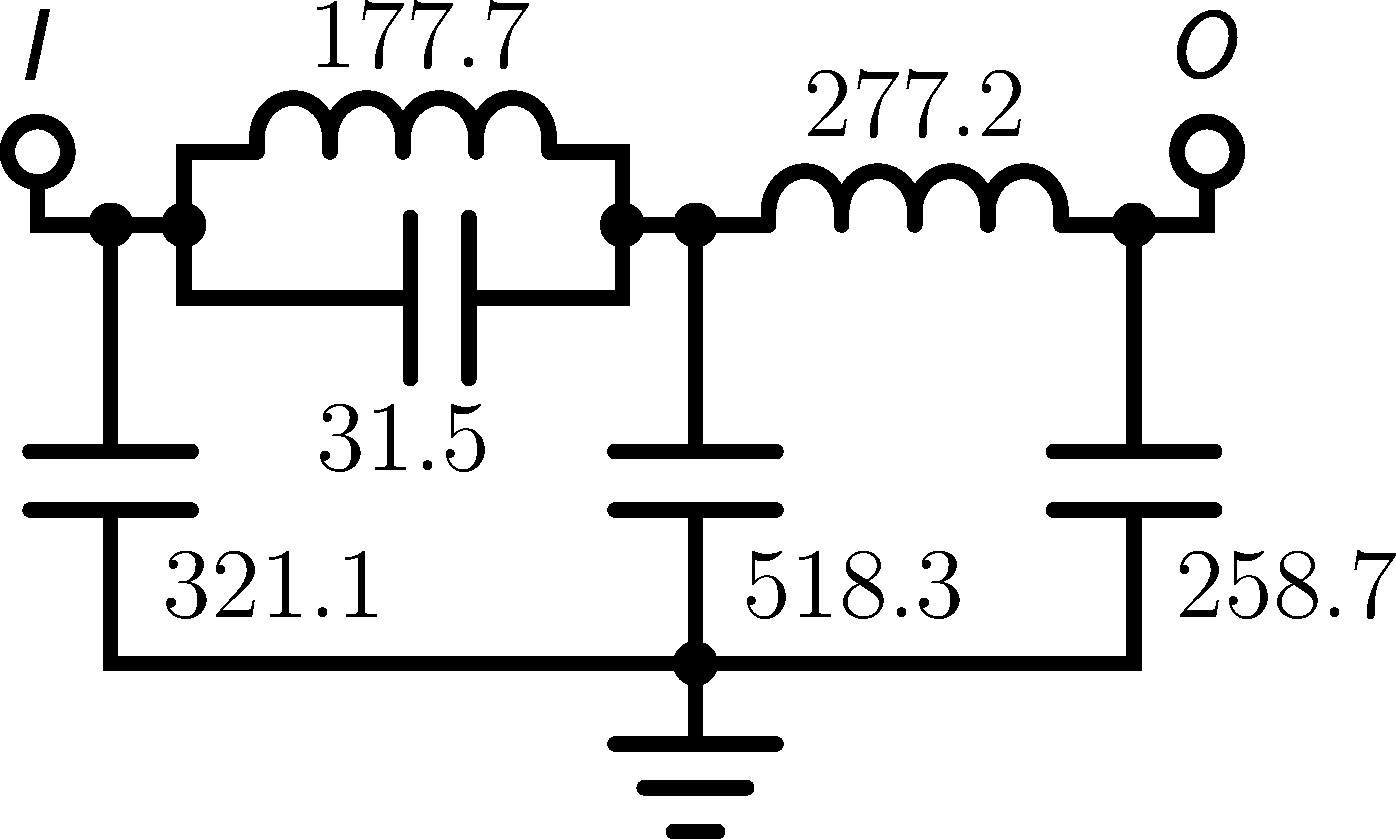
\includegraphics[scale = 0.14]{../ch6/figures/lpf3_circuit1}
\caption{\label{fig:lpf3_circuita}}
\end{subfigure}%
\begin{subfigure}[t]{0.25\textwidth}
\centering
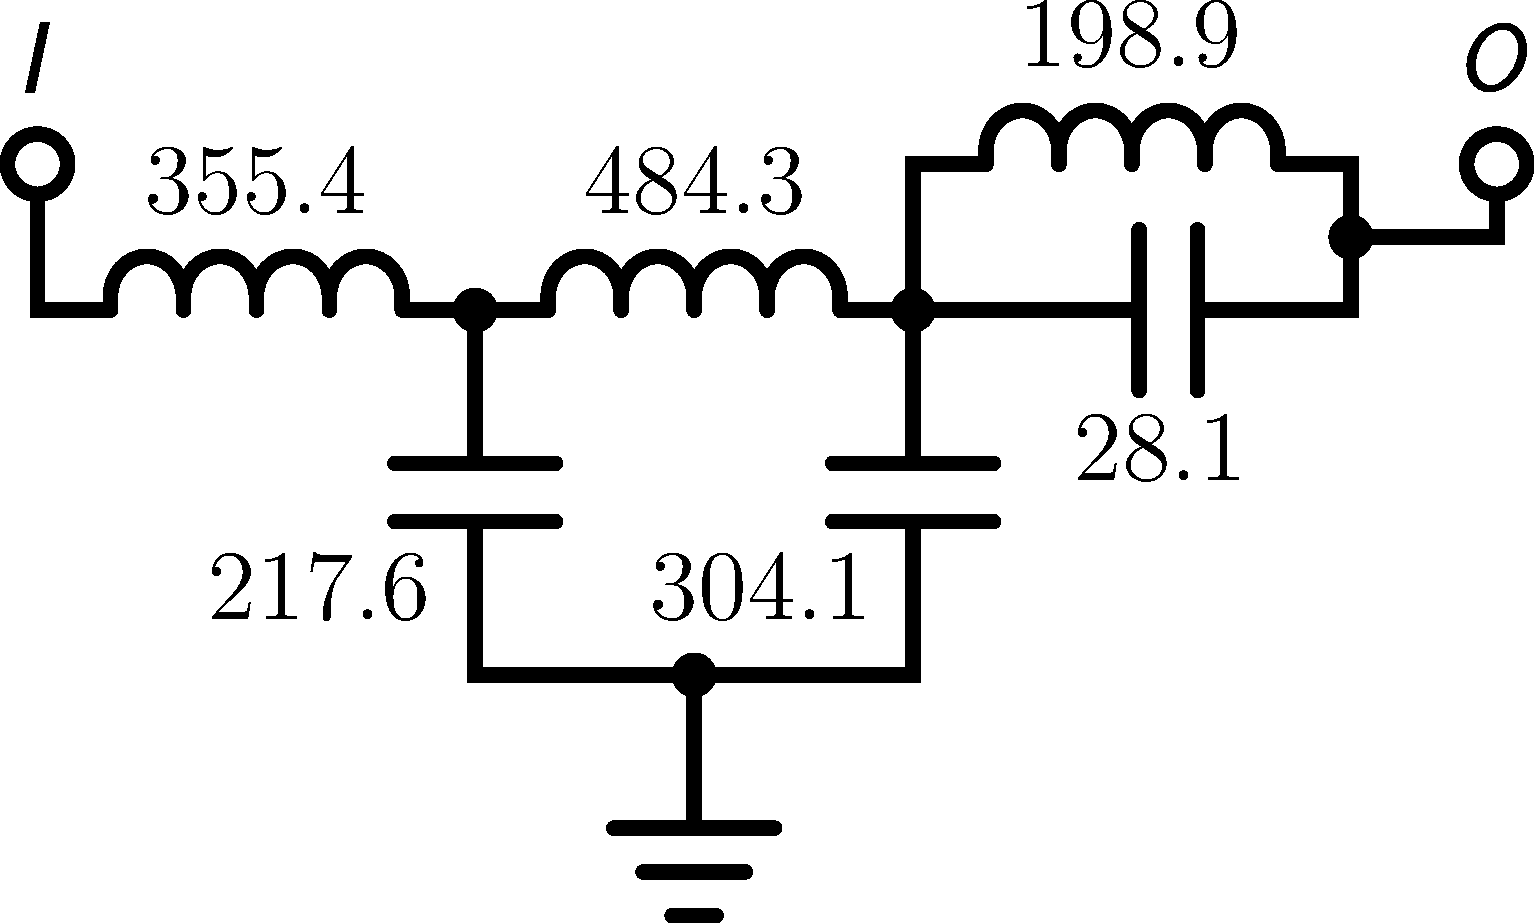
\includegraphics[scale = 0.14]{../ch6/figures/lpf3_circuit2}
\caption{\label{fig:lpf3_circuitb}}
\end{subfigure}%
\begin{subfigure}[t]{0.25\textwidth}
\centering
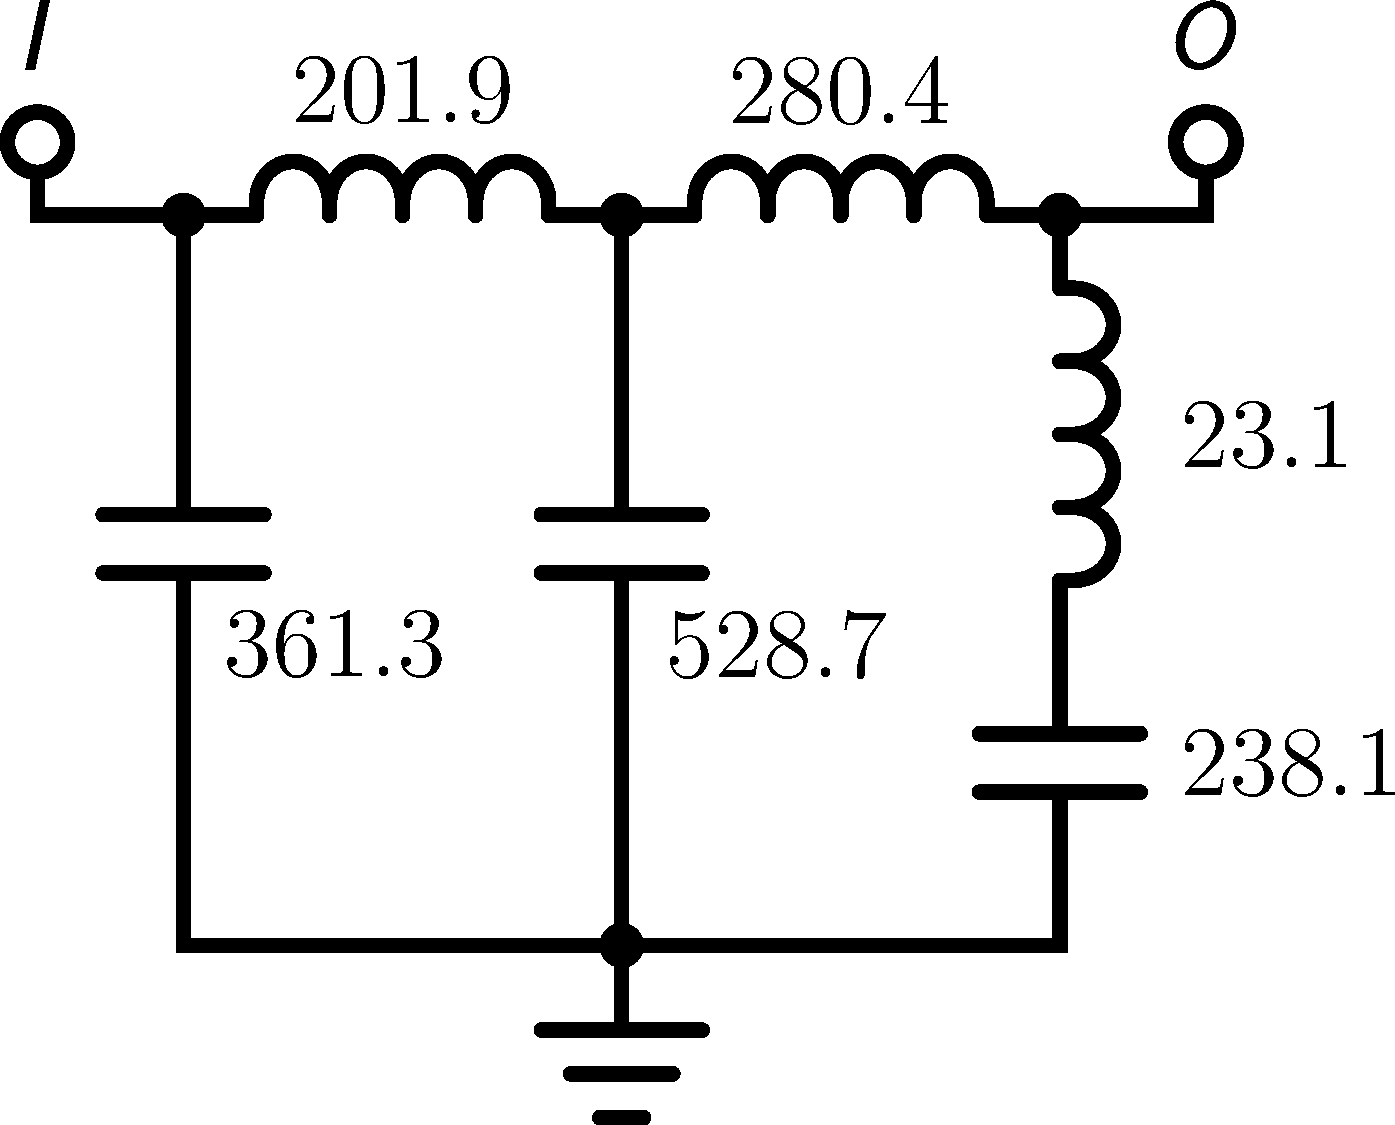
\includegraphics[scale = 0.14]{../ch6/figures/lpf3_circuit3}
\caption{\label{fig:lpf3_circuitc}}
\end{subfigure}%
\begin{subfigure}[t]{0.25\textwidth}
\centering
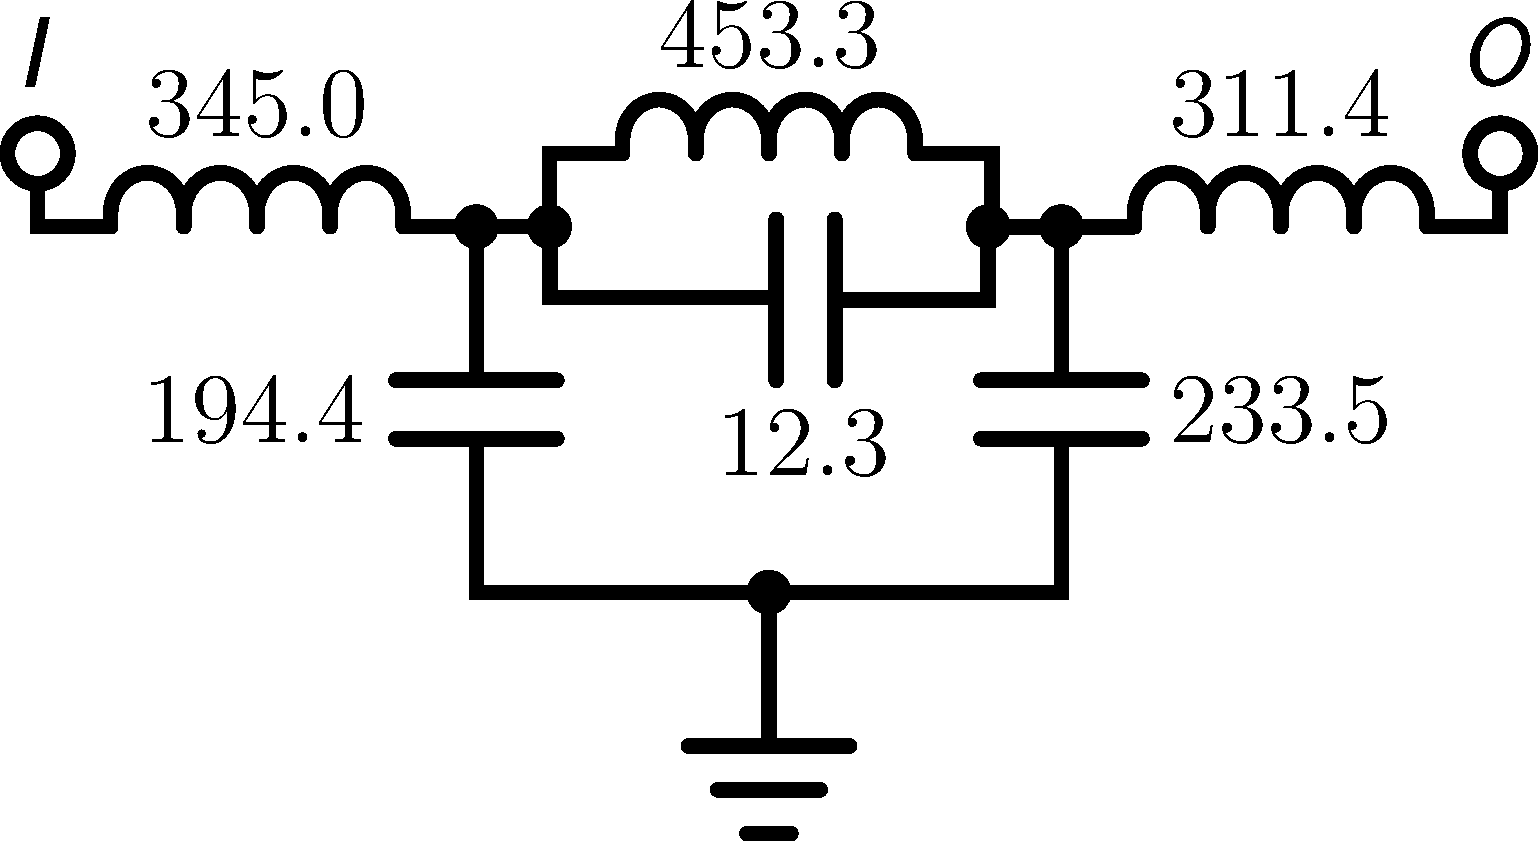
\includegraphics[scale = 0.14]{../ch6/figures/lpf3_circuit4}
\caption{\label{fig:lpf3_circuitd}}
\end{subfigure}%
\vspace{0.06in}
\begin{subfigure}[t]{\textwidth}
\centering
% 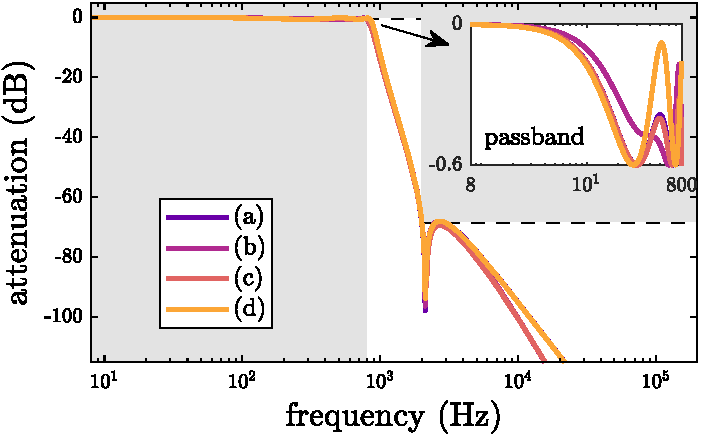
\includegraphics[width=\textwidth]{../ch6/figures/lpf3_magnitude}
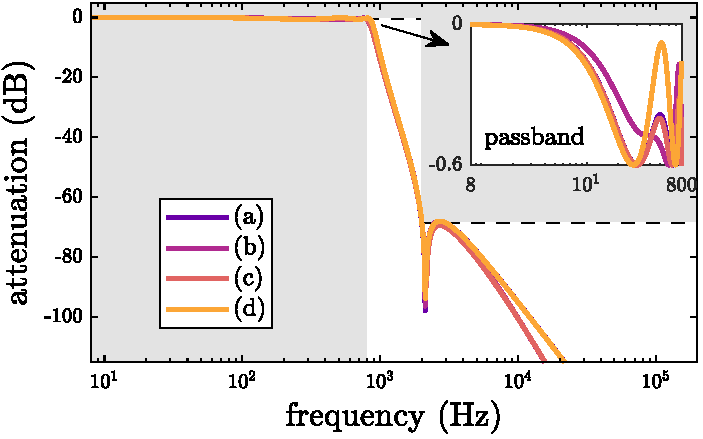
\includegraphics[width=0.5\textwidth]{../ch6/figures/reduced/r_lpf3_magnitude}
\caption{\label{fig:lpf3_magnitude}}
\end{subfigure}%

\caption[Select feasible, minimum complexity circuits and attenuation responses for \nameref{sec:ch6:lpf} task \#3.]{Select feasible, minimum complexity circuits and attenuation responses for \nameref{sec:ch6:lpf} task \#3 (units are mH and nF).\label{fig:lpf3}}

\end{figure}

The next task had slightly more stringent $K_p$ and $K_s$ limits, but the transition region was slightly larger.
Furthermore, the variables bounds are the tightest of the four tasks.
Only 197 topologies where found to be feasible, which is less than with task \#2. 
In this task, six components was the minimum number required, and four of the ten minimum complexity topologies are shown in Figs.~\ref{fig:lpf3_circuita}--\ref{fig:lpf3_circuitd} (all ten circuits are shown in Fig.~\ref{fig:app2:lpf3}). The minimum inductor topology is illustrated in Fig.~\ref{fig:lpf3_circuita}. 
Their attenuation responses are shown in Fig.~\ref{fig:lpf3_magnitude}, and all responses are within the specifications.
The circuit in Fig.~\ref{fig:lpf3_circuitc} is the same topology found in Ref.~\cite{Das2007a}, which is another case of an evolutionary approach arriving at a minimum complexity circuit.

% study 4
\begin{figure}
\centering
\begin{subfigure}[t]{0.3\textwidth}
\centering
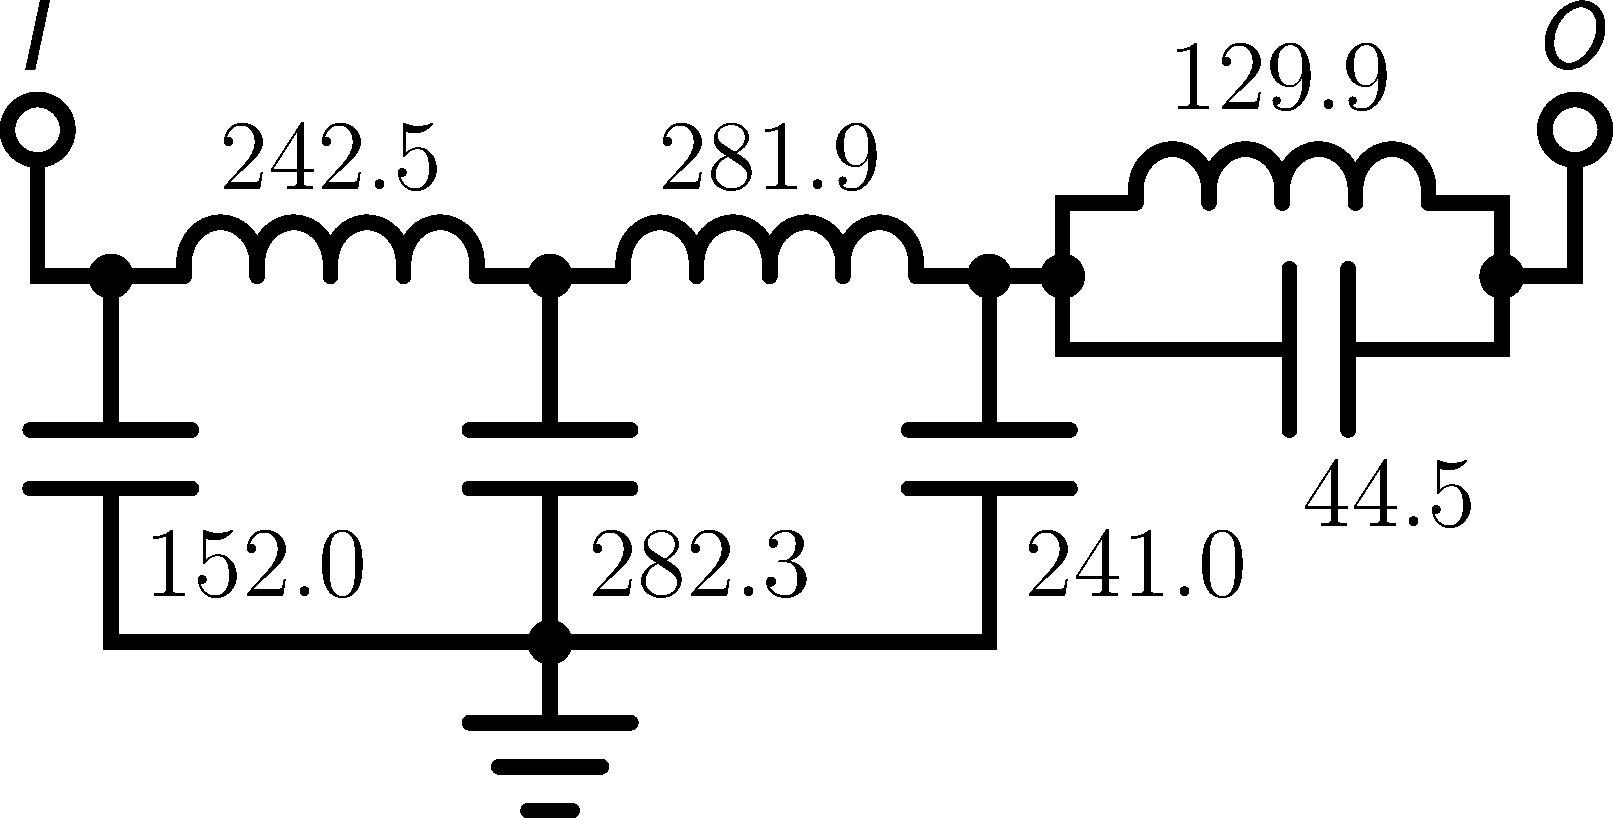
\includegraphics[scale = 0.14]{../ch6/figures/lpf4_circuit1}
\caption{$\{0.0875, 63.08\}$.\label{fig:lpf4_circuita}}
\end{subfigure}%
\begin{subfigure}[t]{0.3\textwidth}
\centering
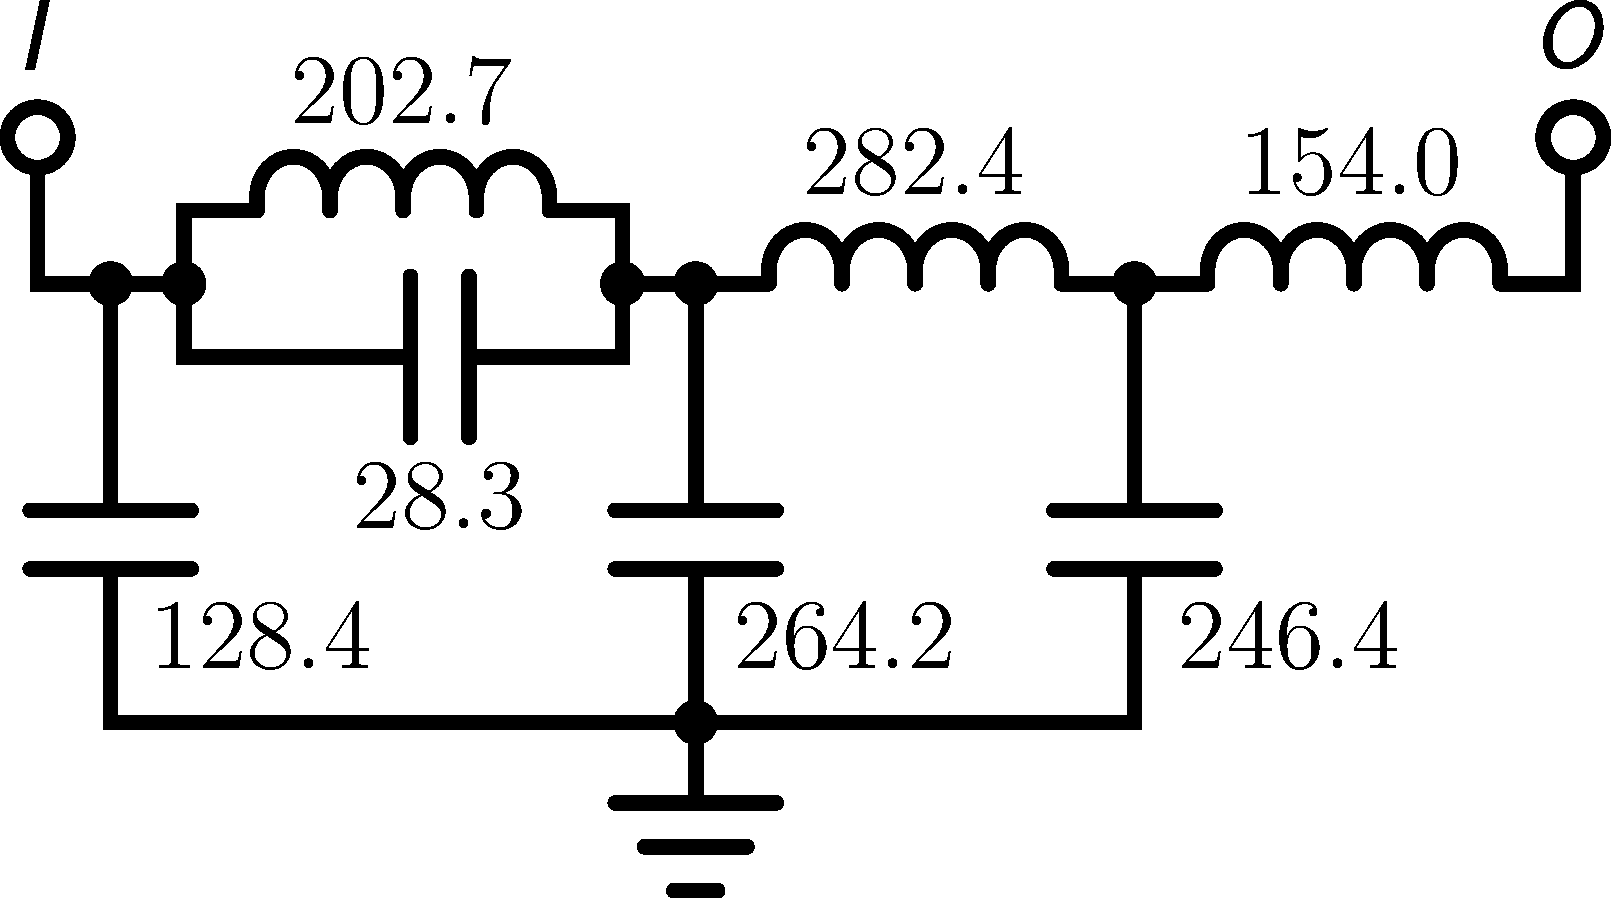
\includegraphics[scale = 0.14]{../ch6/figures/lpf4_circuit2}
\caption{$\{0.1222, 62.92\}$.\label{fig:lpf4_circuitb}}
\end{subfigure}%

\caption[Top two closest to be feasible circuits for \nameref{sec:ch6:lpf} task \#4.]{Top two closest to be feasible circuits for \nameref{sec:ch6:lpf} task \#4 and realized gains $\{K_p,K_s\}$ with respect to $f_p=1000$ Hz and $f_s=2000$ Hz (units are mH and nF).\label{fig:lpf4}}

\end{figure}

Task \#4 had the toughest specifications, primarily due to $K_p = 0.01$.
Since the requirements were equal to or more stringent than those in task \#2, only the 280 feasible circuits from task \#2 were tested, greatly reducing the computational cost. 
None of the topologies produced a feasible circuit, so we come to the conclusion that at least eight components are needed.
In Ref.~\cite{Lohn1999a}, 21 components were needed, but in Ref.~\cite{Goh2001a}, only 12 components.
Therefore, we now know that between 8 and 12 components are required to produce a feasible design.

% new paragraph
The top two circuits (in terms of performance) are shown in Fig.~\ref{fig:lpf4}.
As expected, they both include seven components, which was the limit.
The topologies are similar to minimum complexity topologies found in the previous tasks. 
Fig.~\ref{fig:lpf4_circuita} is similar to Fig.~\ref{fig:lpf3_circuitb}, and Fig.~\ref{fig:lpf4_circuitb} is similar to Fig.~\ref{fig:lpf3_circuita}.
For the best circuit, the gains $\{K_p,K_s\}$ were found to be $\{0.0875, 63.08\}$, which are a substantial improvement compared to task \#2, but still do not meet this task's stringent specifications.